\section{Experimental setup}
\label{sec:design}

We evaluate discovery and closed-loop mitigation in a system-level O-RAN surge simulation, and isolate the role of
the logging design in controlled environments with known causal structure.

\subsection{Simulation environment and scenario}
\label{sec:scenario}\claim{DEF-SIM-CONST}

The simulator models a near-RT RIC and the RAN it controls (Figure~\ref{fig:system}). The network has 24 cells: 21
macro sectors on a seven-site hexagonal layout~\cite{3gpp36814} and three co-channel picos at traffic hotspots, serving
300 UEs in a low-latency (LL), an enhanced mobile broadband (eMBB) or a best-effort slice. Traffic, mobility and a
hidden per-site load process come from an exogenous tape keyed by the seed, so that runs that act differently see the
same tape (parameters in \esm{esm:setup}). In the surge scenario, a localised surge triples the file-arrival rate of the UEs
near a venue during the middle of the scored window.

Three xApps run on the RIC, each writing its own parameter families (Table~\ref{tab:xapps}). The Energy Saving (ES)
xApp switches macro carriers and puts picos to sleep using the load-time thresholds of 3GPP TS 28.541~\cite{3gpp28541},
and the Power ES xApp backs off the macro transmit power as in 3GPP TR 38.864~\cite{3gpp38864}. The Slice Guarantee
xApp sets the protected minimum PRB share that serves a protected subset of the eMBB UEs. The result is a three-way
indirect conflict without a shared parameter: the energy-saving xApps act on the KPIs of neighbouring cells, and Slice
Guarantee on the protected-slice violations of its own cell. The edge from pico sleep to neighbour protected-slice
violations is the one on which the conflict rests: since the protected share moves only its own cell's protected-slice
violations, a referee that rejects Slice Guarantee's requests removes the protection that the energy-saving xApps
erode.

\begin{table}[tbp]
\caption{xApps of the surge scenario.}
\label{tab:xapps}
\setlength{\tabcolsep}{4pt}
\begin{tabular}{@{}p{2.2cm} p{3.5cm} p{3.0cm} p{3.5cm}@{}}
\toprule
xApp & Parameter & Range & Acts when \tabularnewline
\midrule
\raggedright ES & \raggedright Macro carrier; pico sleep & \raggedright on/off; awake/asleep & \raggedright load low / high \tabularnewline
\raggedright Power ES & \raggedright Macro transmit-power offset & \raggedright $-9$ to 0~dB & \raggedright load low / high \tabularnewline
\raggedright Slice Guarantee & \raggedright Protected minimum PRB share & \raggedright 0 to 0.5 & \raggedright protected UEs below floor \tabularnewline
\bottomrule
\end{tabular}
\end{table}

\subsection{Datasets}
\label{sec:datasets}\claim{PRO-TUNE}

Discovery uses uniform-randomised and state-dependent logs of 600 evaluation episodes each, matched placebo logs, and
null outcomes formed by cyclically shifting KPI series across episodes. Unlike placebos, the null outcomes retain the
re-proposals and state-dependent propensities. Maps learned from the state-dependent logs drive ungated and gated
referees on separate fresh seeds; the gate is calibrated on \val{s3.gate.dev_episodes} development episodes. All
methods and baseline thresholds are tuned on development episodes separate from evaluation.

\subsection{Knockout ground truth}
\label{sec:gt}\claim{DEF-GT-LABEL}

The maps are scored against knockout rollouts, which estimate the effect of one unit's mode with every other unit
accepted; as this target is not PMRT's $\tau_{\pi}$, the scores measure agreement rather than the validity of the
test.

\begin{definition}[Knockout effect]
\label{def:tau_aa}\claim{DEF-EST-TAUAA}
Let $u$ be a unit sampled on separate episodes. Its knockout effect $\tau_u^{\mathrm{AA}}$ is the accept-minus-reject
difference of the KPI summed over the cells of $r$ in the 90~s after opening, in rollouts from the copied state with
every other unit accepted. The knockout effect $\tau_{\mathrm{AA}}$ is the mean of $\mathrm{sgn}_u\,
\tau_u^{\mathrm{AA}}$ over the sampled units.
\end{definition}

Pooling the units of a family over \val{s1.gt.episodes} ground-truth episodes gives a mean per hypothesis with a 95~\%
episode-cluster bootstrap interval. A hypothesis is labelled true, with the sign of its mean, when the interval
excludes zero and the absolute mean is at least a materiality threshold $\delta_k$, set to 5~\% of the largest
absolute mean of KPI $k$. It is labelled knockout-null when the interval lies within $\pm\delta_k$, and is otherwise
left unscored. This is a practical-equivalence label rather than PMRT's sharp null (Table~\ref{tab:terms}), and it
depends materially on $\delta_k$ (\esm{esm:discovery}). On the uniform-randomised logs the ground truth labels 29 of the 60 hypotheses true, 21 null and 10
indeterminate (\esm{esm:setup}).\claim{EMP-GT-LABELS}

\subsection{Controlled environments}
\label{sec:envs}\claim{DEF-ENV}\claim{DEF-ENV-ARMS}\claim{ASM-S4-KNOWN}

The simulator runs one scenario with one logging design per dataset, and its ground truth is estimated. The controlled
environments remove both limitations: each isolates one mechanism with a known causal graph, so that every null edge
is null by construction, and the same mechanism is logged under several designs. The five environments contain a
clean linear graph, an edge active only in a rare regime, delayed harm through lagged KPI cascades, latent
confounding, and the three mechanisms composed (Figure~\ref{fig:envs}a). Actions are logged by independent redraws per
observation, by a dithered setpoint held for a twentieth of the data plus a small independent dither, or, in the
latent-confounding environment, by a confounded behaviour policy with logged probabilities (Figure~\ref{fig:envs}b).
Each method ran at 500 to 24\,000 observations, and each condition on 40 seeds. A null-edge rate is invalid when the
lower bound of its 95~\% seed-cluster bootstrap interval exceeds 0.05, valid when the upper bound is at most 0.075, and
inconclusive otherwise; a condition is invalid when any of its rates is.

\begin{figure}[tbp]
\centering
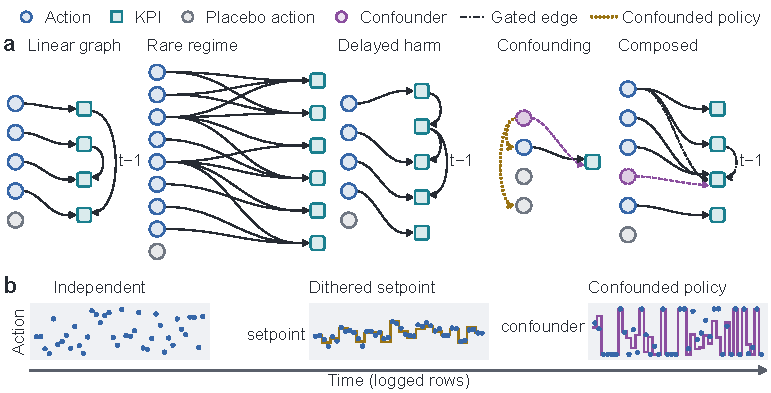
\includegraphics[width=\textwidth]{figures/fig_envs.pdf}
\caption{Controlled environments and logging designs.}
\label{fig:envs}
\end{figure}

Three groups of tests are compared. Design-based tests redraw the logged design: PMRT-GBM, which uses a
gradient-boosting statistic and plain BY control at $q = 0.05$, and its linear counterpart PMRT-Lin.
Design-adjusted tests condition on the logged design variables: partial correlation, Granger and
RCoT~\cite{strobl2019rcot}. Design-blind methods ignore those variables: correlation; partial correlation
with standard or heteroskedasticity- and autocorrelation-consistent errors~\cite{newey1987hac,kiefer2005fixedb};
Granger; RCoT; PC~\cite{spirtes2000causation}; NOTEARS~\cite{zheng2018notears}; SHAP-DAG after Sharma et
al.~\cite{Sharma_2025,lundberg2017shap}; the two-tower network; our earlier max-stratified
correlation-ratio test; and CDD O-RAN's discovery stage~\cite{dahal2026cddoran}. These environments isolate
the randomisation construction shared by the PMRT variants, not the simulator PMRT's matched-filter
statistic or weighted declaration layer; its validity therefore rests on the simulator null checks in
Section~\ref{sec:res_validity}.

\subsection{Baselines and metrics}
\label{sec:baselines_scores}\claim{DEF-MET-MAP}\claim{DEF-MET-DEC}

In the simulator, PMRT is compared with seven associational baselines that ignore the logging design and run on the
same unit table (\esm{esm:setup}): correlation, Granger~\cite{granger1969causal} with a tuned threshold or under BY control
(Granger~+~BY), SHAP-GBDT~\cite{Sharma_2025}, a two-tower network~\cite{santos2026conflictairan}, the intent-conflict
statistic INT of PACIFISTA~\cite{PACIFISTA} and QACM~\cite{QACM2024}. Each threshold was set on development episodes so
that the far relation received at most one declaration. Because the ground truth labels \val{s1.far.true} of the
\val{s1.far.total} far hypotheses true on the uniform-randomised logs and \val{s2.far.true} on the state-dependent logs, this rule
caps the recall a baseline can reach. On the uniform-randomised logs the baselines' placebo declarations come from their
thresholds rather than from confounding, and on the state-dependent logs the baselines are also reported at thresholds
calibrated on placebo logs.

Maps are scored over the \val{s1.gt.hypotheses} hypotheses; indeterminate labels count in neither precision nor
recall, F1 is their harmonic mean, and sign accuracy is the share of declared true edges with the ground-truth sign.
Referees are compared with accept-all, never-sleep, single-xApp subsets, and referees driven by the oracle, random and
associational maps (\esm{esm:setup}). Protected-slice violations $V$ define the recovery
$R = (V_{\mathrm{AA}} - V)/(V_{\mathrm{AA}} - V_{\mathrm{ref}})$, which is 0 for accept-all and 1 for the best
single-xApp subset. Eligibility requires the constraints of Section~\ref{sec:estimand}; never-sleep is the best
eligible static rule because the subset attaining $R = 1$ retains almost no energy saving. Decision intervals are
90~\% paired seed-bootstrap intervals and rate intervals are 95~\% cluster-bootstrap intervals.
